\section*{Results}

\begin{figure}[H]
  \centering
  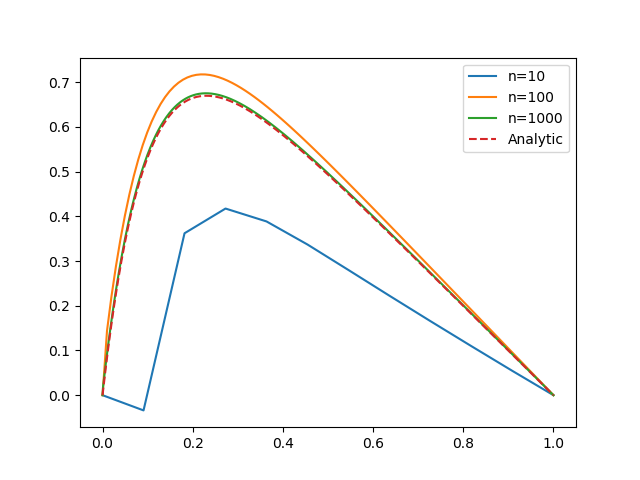
\includegraphics[width=\textwidth]{../figures/thomas.png}
  \caption{Comparison of analytic solution and numerical approximations}
  \label{fig:a}
\end{figure}


The thomas algorithm run time \cref{table:thomas} is roughly linear with the
matrix size.

\begin{table}[h]
  \centering
  \csvautotabular{../data/thomas.csv}
  \caption{Run times of thomas algorithm for selected matrix sizes.}
  \label{table:thomas}
\end{table}

The improved thomas algorithm \cref{table:toeplitz} run time is in the same
order of magnitude as the normal thomas algorithm, but consequently a bit faster.

\begin{table}[h]
  \centering
  \csvautotabular{../data/toeplitz.csv}
  \caption{Run times of improved thomas algorithm when considering a töeplitz matrix.}
  \label{table:toeplitz}
\end{table}

\begin{table}[h]
  \centering
  \csvautotabular{../data/relative_error.csv}
  \caption{Maximum relative error between analytic and numeric solution.}
  \label{table:relative_error}
\end{table}

Comparing the run times using LU decomposing and backward substituting
(\cref{table:LU_timing}) with run times using the thomas algorithm
(\cref{table:thomas}) we see that the thomas algorithm is roughly n times
faster.

\begin{table}[h]
  \centering
  \csvautotabular{../data/LU_timing.csv}
  \caption{Run time for solving $A\bvec{x} = \bvec{b}$ by LU decomposing and backward substituting.}
  \label{table:LU_timing}
\end{table}
